%% ****** Start of file apstemplate.tex ****** %
%%
%%
%%   This file is part of the APS files in the REVTeX 4 distribution.
%%   Version 4.1r of REVTeX, August 2010
%%
%%
%%   Copyright (c) 2001, 2009, 2010 The American Physical Society.
%%
%%   See the REVTeX 4 README file for restrictions and more information.
%%
%
% This is a template for producing manuscripts for use with REVTEX 4.0
% Copy this file to another name and then work on that file.
% That way, you always have this original template file to use.
%
% Group addresses by affiliation; use superscriptaddress for long
% author lists, or if there are many overlapping affiliations.
% For Phys. Rev. appearance, change preprint to twocolumn.
% Choose pra, prb, prc, prd, pre, prl, prstab, prstper, or rmp for journal
%  Add 'draft' option to mark overfull boxes with black boxes
%  Add 'showpacs' option to make PACS codes appear
%  Add 'showkeys' option to make keywords appear
\documentclass[aps,prl,groupedaddress,twocolumn]{revtex4-1}
%\documentclass[aps,prl,preprint,superscriptaddress]{revtex4-1}
%\documentclass[aps,prl,reprint,groupedaddress]{revtex4-1}

\usepackage{graphicx}
\usepackage{epsfig}
\usepackage{subcaption}

\usepackage{amsmath}
\usepackage{amssymb}

\usepackage{dsfont}
\usepackage{bm}
\usepackage{slashed}
\usepackage{cancel}

%package for highlighting text
\usepackage[dvipsnames]{xcolor}
\usepackage{soul} % use \hl{} to highlight text

\usepackage{feynmp}
\usepackage{tikz}
\usepackage{tikz-feynman}
\tikzfeynmanset{
  fermion1/.style={
    /tikz/postaction={
      /tikz/decoration={
        markings,
        mark=at position 0.5 with {
          \node[
            transform shape,
            xshift=-0.5mm,
            fill,
            dart tail angle=100,
            inner sep=1.8pt,
            draw=none,
            dart
          ] { };
        },
      },
      /tikz/decorate=true,
    },
  }
}

%list of my new commands
\newcommand{\beq}{\begin{equation}}

\newcommand{\eeq}{\end{equation}}

\newcommand{\eq}[1]{\begin{equation}\begin{aligned}#1\end{aligned}\end{equation}}

\newcommand{\eqs}[1]{\begin{equation*}\begin{split}#1\end{split}\end{equation*}}

\newcommand{\pp}[2]{\frac{\partial #1}{\partial #2}}

\newcommand{\pa}{\partial}

\newcommand{\da}{\text{d}}

\newcommand{\pd}[2]{\frac{\text{d}#1}{\text{d}#2}}

\newcommand{\Lra}{\Leftrightarrow}

\newcommand{\lra}{\leftrightarrow}

\newcommand{\la}{\leftarrow}

\newcommand{\ra}{\rightarrow}

\newcommand{\Ra}{\Rightarrow}

\newcommand{\La}{\Leftarrow}

\newcommand{\ve}{\varepsilon}

\newcommand{\ttt}[1]{\texttt{#1}}

\newcommand{\R}{\mathds{R}}

\newcommand{\ricci}{\text{\textsc{R}}}

\newcommand{\vp}{\varphi}

\newcommand{\vs}{\varsigma}

\newcommand{\ordo}{\mathcal{O}}

\newcommand{\ham}{\mathds{H}}

\newcommand{\p}{\mathds{P}}

\newcommand{\vk}{\varkappa}

\newcommand{\MF}{\mathcal{F}}

\newcommand{\MS}{\mathcal{S}}

\newcommand{\ML}{\mathcal{L}}

\newcommand{\MJ}{\mathcal{J}}

\newcommand{\MA}{\mathcal{A}}

\newcommand{\cd}{\cdot}

\newcommand{\dgr}{^\dagger}

\newcommand{\pref}[1]{(\ref{#1})}

\makeatletter
\newcommand{\vast}{\bBigg@{4}}
\newcommand{\Vast}{\bBigg@{5}}
\newcommand{\VVast}{\bBigg@{8}}
\makeatother

% You should use BibTeX and apsrev.bst for references
% Choosing a journal automatically selects the correct APS
% BibTeX style file (bst file), so only uncomment the line
% below if necessary.
%\bibliographystyle{apsrev4-1}

\begin{document}

% Use the \preprint command to place your local institutional report
% number in the upper righthand corner of the title page in preprint mode.
% Multiple \preprint commands are allowed.
% Use the 'preprintnumbers' class option to override journal defaults
% to display numbers if necessary
%\preprint{}

%Title of paper
\title{Temperature Comparisons Between Lund, Uppsala, and Luleå}

% repeat the \author .. \affiliation  etc. as needed
% \email, \thanks, \homepage, \altaffiliation all apply to the current
% author. Explanatory text should go in the []'s, actual e-mail
% address or url should go in the {}'s for \email and \homepage.
% Please use the appropriate macro foreach each type of information

% \affiliation command applies to all authors since the last
% \affiliation command. The \affiliation command should follow the
% other information
% \affiliation can be followed by \email, \homepage, \thanks as well.
\author{Emil Boman}
\email[Emil Boman: ]{nat14ebo@student.lu.se}
\author{Henrik Olsson}
\email[Henrik Olsson: ]{he4511ol-s@student.lu.se}
\author{Pavel Oshchepkov}
\email[Pavel Oshchepkov: ]{paul.oshchepkov@icloud.com}
%\homepage[]{Your web page}
%\thanks{}
%\altaffiliation{}
%\affiliation{}

%Collaboration name if desired (requires use of superscriptaddress
%option in \documentclass). \noaffiliation is required (may also be
%used with the \author command).
%\collaboration can be followed by \email, \homepage, \thanks as well.
%\collaboration{}
%\noaffiliation

\date{\today}

\begin{abstract}

\end{abstract}

\maketitle


\section{\label{intro}Introduction}


%Things to add here:
%\begin{itemize}\setlength\itemsep{-0.2cm}
%    \item Intro to subject
%    \item some background
%    \item goals
%    \item introduce the datasets and their characteristics (particularly important for Lund, were the number of measurements per day varies).
%    \item what was done (remember to include info about choice of git setup)
%    \item short about results
%    \item structure of the report.
%\end{itemize}



In this project we explore a number of long term temperature comparisons between Lund, Uppsala, and Luleå. The first of these is the number of winter days per year. This both includes studying the change in absolute numbers over time, and the relative change between the cities. The second is the average monthly temperature difference between Lund and Luleå, and in order to obtain this the average monthly temperature for both cities was determined. The third comparison is the hottest and coldest day of the year, where the number of times each day of the year has been the hottest or coldest is shown for each of the three cities.

The datasets, in the form of comma separated values (CSV) files, used for these comparisons were taken from SMHI open data \cite{smhi}. The Luleå dataset contains hourly measurements going back to 1949. For the same time period the Uppsala dataset also contains hourly measurements. In contrast, the Lund dataset varies between two, three, and five measurments per day during the time period. Table \ref{tab:lund_meas_struct} shows the time of day measurements where taken in the Lund dataset from 1949 to 2023.

\begin{table}[h!]
    \centering
    \begin{tabular}{c|c}
        Time Period & Time of Measurements\\
        \hline
        1949$\ra$ 1974-05-31 & 06:00, 12:00, and 18:00 \\
        \hline
        1974-06-01$\ra$1980-02-29 & 06:00, 09:00, 12:00, 15:00 and 18:00\\
        \hline
        1980-03-01$\ra$1996-06-30 &  06:00, 12:00, and 18:00 \\
        \hline
        1996-07-01$\ra$ & 06:00 and 18:00\\
        \hline
    \end{tabular}
    \caption{The time of day measurements were made for different time periods in the Lund dataset.}
    \label{tab:lund_meas_struct}
\end{table}

Concerning the git-policy used for this project, all developers were allowed to directly interact with the main repository. The reason for this choice was that developers were working at different parts of the project, and had differing working hours, making it the most convenient policy for a short-term project.

The structure of the remainder of the report is as follows. First, the data cleaning procedure common to all subprojects will be described. After which, the subprojects will be presented one by one. For each of these, data preparation, processing, and plotting will be described, before the results are shown and discussed. Lastly, conclusions and outlook are given. %change to just conclusions if we don't include any outlook.


%%%%%%%%%%%%%%%%%%%%%%%%%%%%%%%%%%%%%%%%%%%%%%%%%%%%%%%%%%%%%%%%%%%%%
\section{Data Cleaning}

The datasets, in the form of csv-files, treated in this project contain meta data that need to be removed from the versions given as input to the data processing functions. In order to accomplish this a simple bash script cleanData.sh was used. It first uses the cut command to separate the first 3 columns in the file, which contain data on the format year;time;temperature. It then uses the tail command to to remove metadata at the top of the file.
\vspace{-0.6cm}
%%%%%%%%%%%%%%%%%%%%%%%%%%%%%%%%%%%%%%%%%%%%%%%%%%%%%%%%%%%%%%%%%
\section{Number of Winter Days}
%intro, restate goal, present structure of section

The aim of this part of the project was to compare the number of winter days, i.e. the number of days with negative average temperature, per year in Lund, Uppsala, and Luleå, during the time period 1964-2022. To accomplish this the number of winter days were calculated and plotted, together with the corresponding centralized moving average over five-year intervals. In addition the relative number of winter days for Lund and Uppsala, using Luleå as the base line, was also determined. The data processing consisted of both a bash script and C++ functions, and the plotting was done using the ROOT framework. In this section begins with a description of the pre-C++ data processing, followed by the C++ data processing and plotting, after which the results are described and analyzed.  
\vspace{-0.5cm}

\subsection{Pre-C++ Data Processing}

The first step of the data treatment, after the cleaning process, is the extraction of days with negative temperature, which is done using the bash script negTempDays.sh . This script also introduces the cut off year 1964. This step reduces the size of the datasets to be treated significantly. Similarly to cleanData.sh, the tail command is utilized to do the line cut off. The grep and sort -u commands are then used to track the days with negative temperatures, which are lastly extracted, again using grep.
\vspace{-0.5cm}

\subsection{C++ Data Processing and Plotting}

The data processing using C++ is done using the functions \texttt{winterday\_map} and \texttt{winterday\_hist\_fill} in \texttt{winterdays}. The first of these take a csv-file on the format \texttt{date,time,temperature} and determines the number of winter days for each year by calculating the number of days where the sum of the temperature measurements are negative, which corresponds to days with negative average temperatures. The number of winter days for each year is then given as output inside a \texttt{map$<$int year,int temperature$>$}. The second function, \texttt{winterday\_his\_fill}, is then used to insert the data in these maps into the corresponding histogram, and to calculate the centralized moving average over five-year intervals, which is also stored in a histogram.

The plotting of the number of winter days histograms is treated by \texttt{winterday\_hist\_draw}, which draws histograms and moving averages, provided in two vectors, on a canvas and then saves the canvas as a pdf. For the plotting of relative number of winter day histograms, \texttt{rel\_winterday\_hist\_gen} is used. This function takes two maps containing years with corresponding number of winter days and inserts the quotient of the number of days into a histogram, using the years as bins. The histogram is then drawn on a canvas, which is saved to a pdf.
\vspace{-0.5cm}

\subsection{Results}

The number of winter days per year recorded in Lund, Uppsala, and Luleå, from 1964 to 2022, is shown as histograms in figure \ref{fig:winterdays}. Included in the figure is also the centralized moving average over five-year intervals for each histogram. 
\vspace{-0.3cm}

\begin{figure}[h!]
    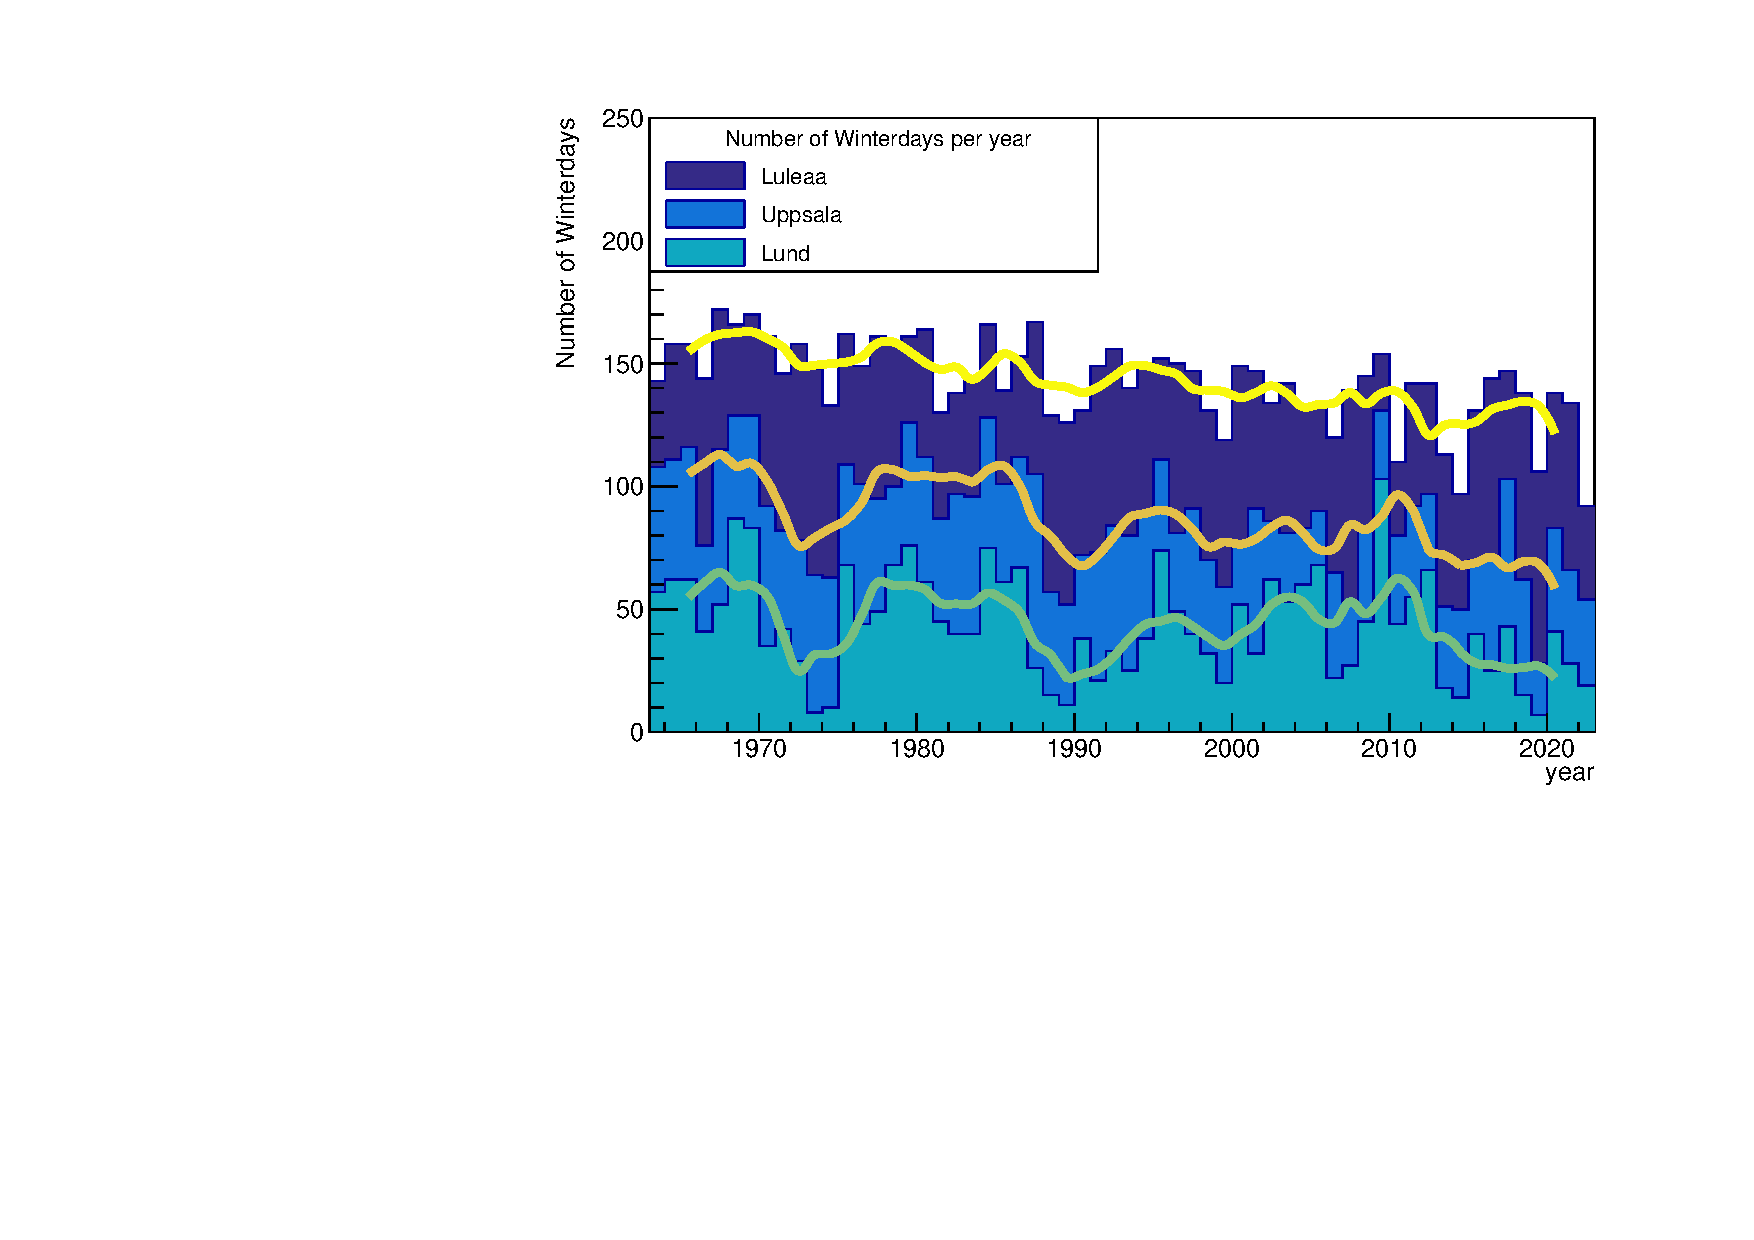
\includegraphics[scale=0.5,trim=0.5cm 0.3cm 0.5cm 1cm,clip]{winterday_hist.pdf}
    \vspace{-0.6cm}
    \caption{The number of winter days from 1964 to 2022 for Lund, Uppsala, and Luleå. The lines are the centralized running average over five-year intervals for the corresponding histogram.}
    \label{fig:winterdays}
\end{figure}

As expected the further north a city is located, the more winter days it tends to have. In addition, the relative variation in number of winter days decreases, and the periods of relatively few winter days shortens, for cities further north. Considering the moving average for Uppsala and Luleå, they show a clear decrease over time, indicating the increase in average temperatures due to global warming. This decrease is not as clear for Lund.

In Lund and Uppsala there was a significant spike in the number of winter days in 2009, after which there has been a period of relatively few winter days, particularly for Lund. It should be noted that Uppsala has had two smaller spikes during this period. Luleå, on the other hand, does not display a similar period. 

The relative number of winter days between Lund and Luleå, from 1964 to 2022, is shown in figure \ref{fig:rel_lund}, and the counterpart for Uppsala is shown in figure \ref{fig:rel_uppsala}. The 2009 spikes are also noticeable in the relative plots, particularly for Lund. Periods of fewer winter days shown in figure \ref{fig:winterdays} have corresponding periods in the relative number of winter days as well, clarifying the higher variation in number of winter days for cities further south. When comparing figures \ref{fig:rel_lund}
and \ref{fig:rel_uppsala}, the higher variation for Lund is also clear.
\vspace{-0.3cm}

\begin{figure}[h!]
    \begin{subfigure}{0.45\textwidth}
            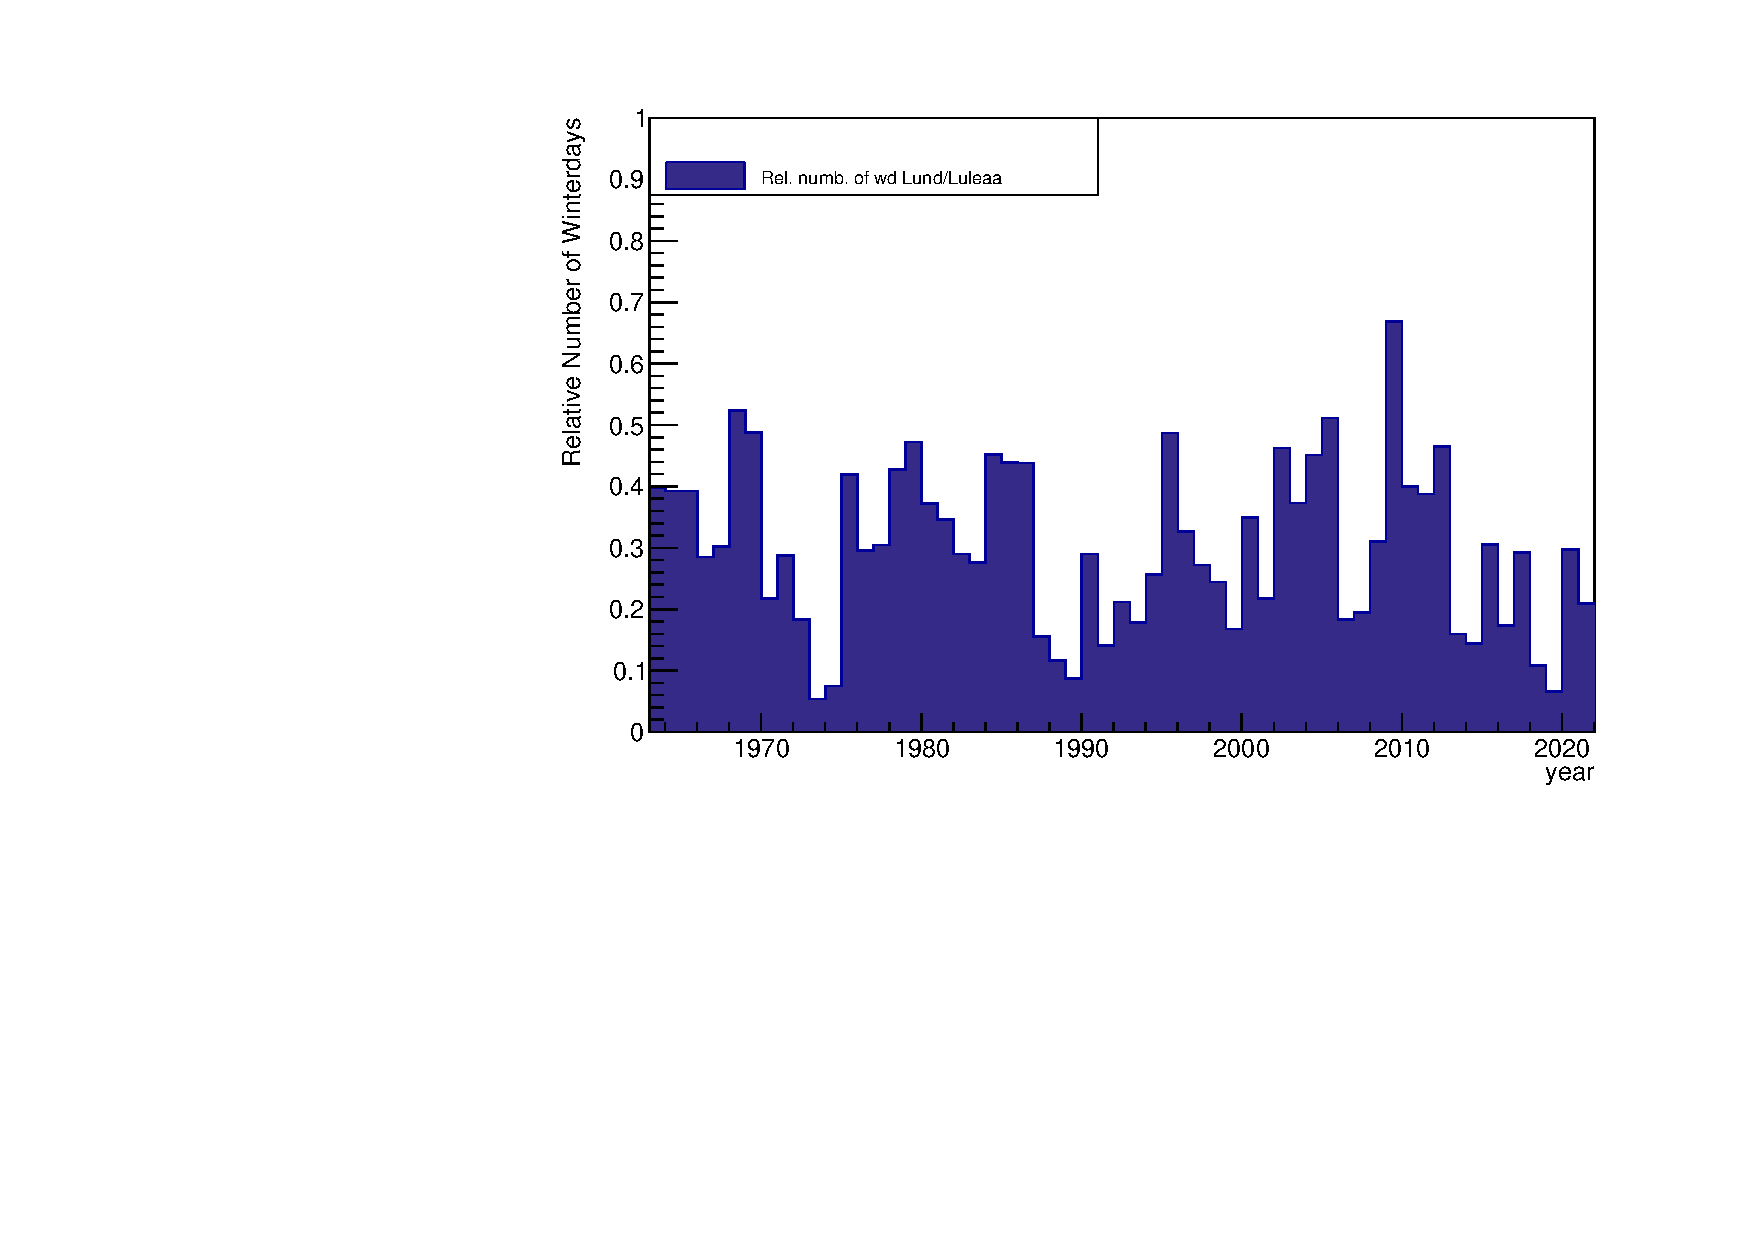
\includegraphics[width=\textwidth,trim= 0 0 0 0.5cm,clip]{rel_Lund_hist.pdf}
            \caption{The relative number of winter days between Lund and Luleå from 1964 to 2022.}
            \label{fig:rel_lund}
    \end{subfigure}

    \vspace{-0.2cm}
    \begin{subfigure}{0.45\textwidth}
            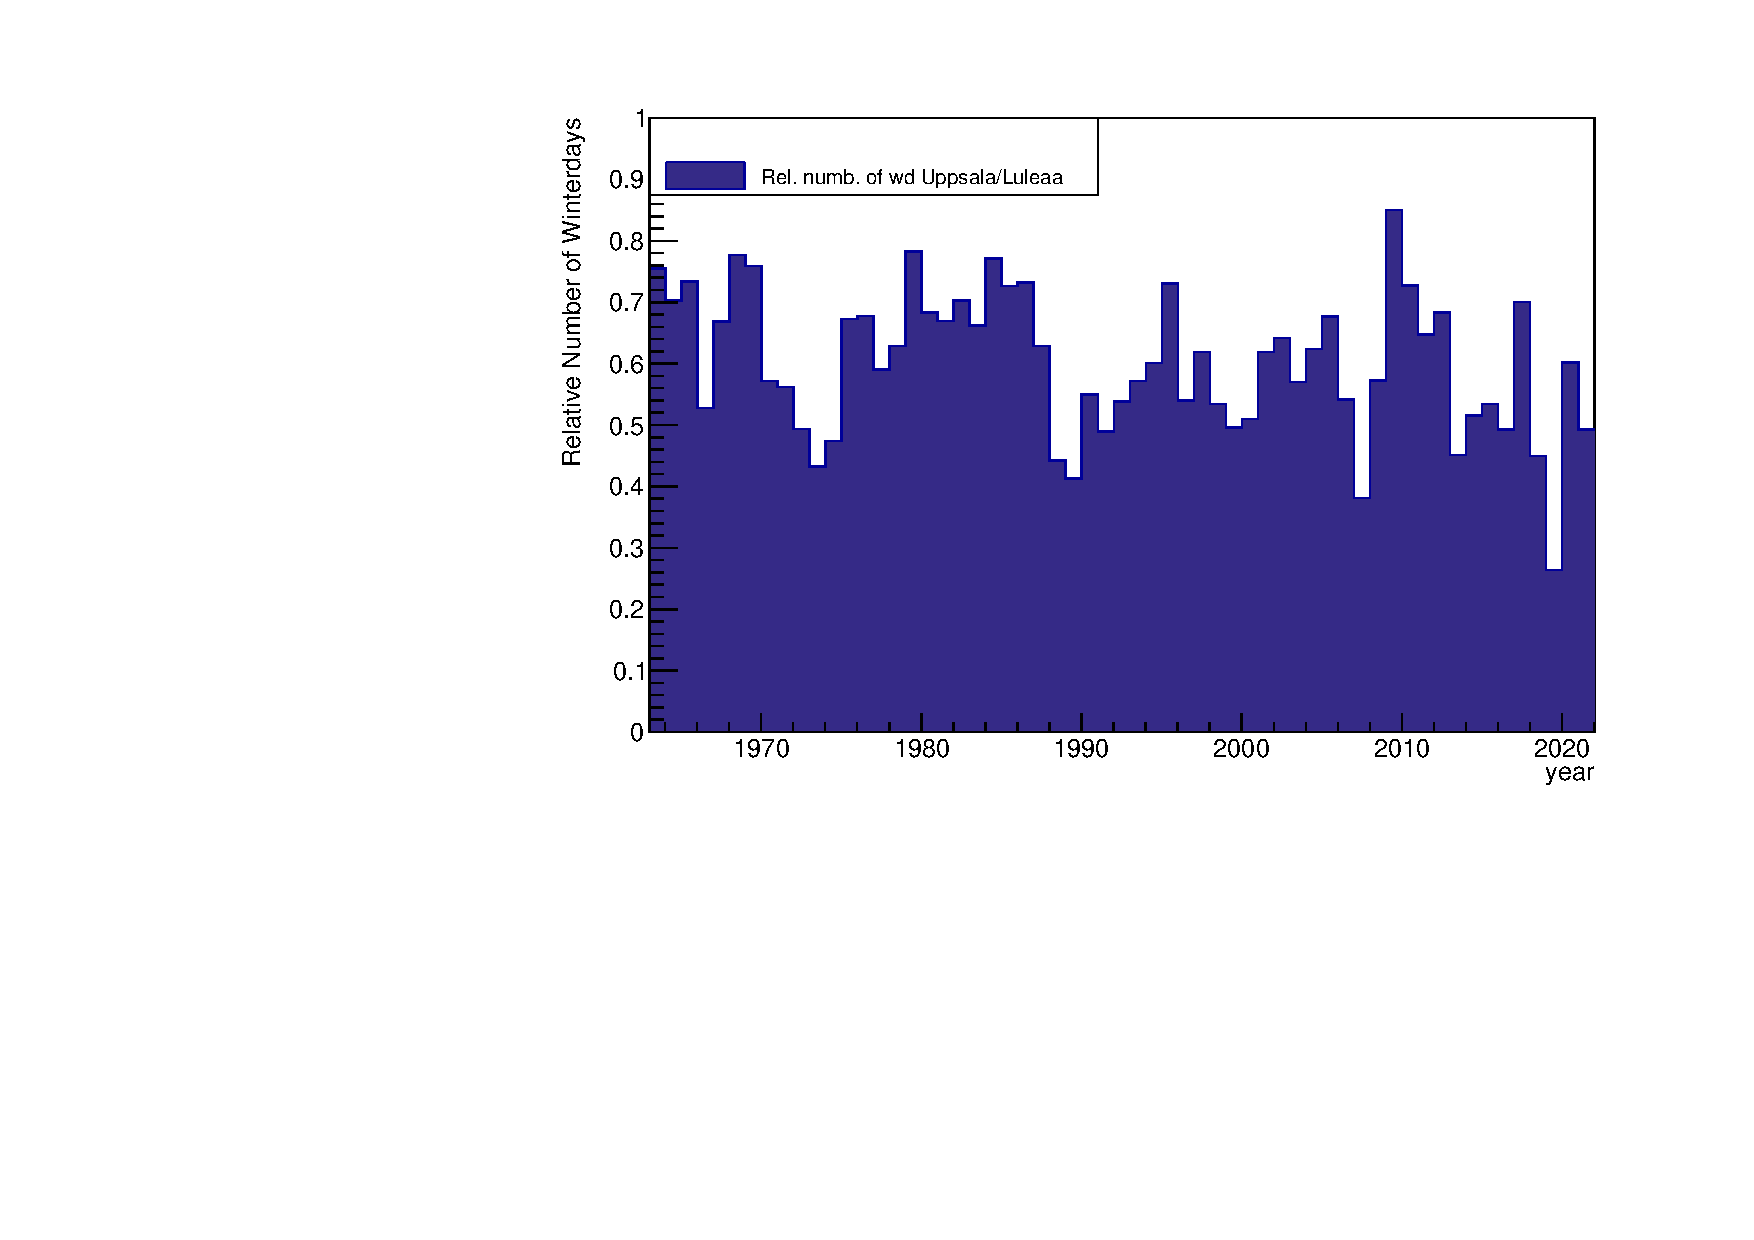
\includegraphics[width=\textwidth,trim= 0 0 0 0.5cm,clip]{rel_Uppsala_hist.pdf}
            \caption{The relative number of winter days between Uppsala and Luleå from 1964 to 2022.}
            \label{fig:rel_uppsala}
    \end{subfigure}
    \caption{The relative number of winter days with Luleå as a reference.}
    \label{fig:rel_winterdays}
\end{figure}
\vspace{-0.2cm}

Considering the quality of the data, it is important to note that while Uppsala and Luleå have temperature measurements taken every hour Lund has measurements with varying intervals during the considered time period (2, 3, and 5 times per day). With fewer measurements the uncertainties in the number of winter days increases, since the calculations of average daily temperatures become much less precise.

%%%%%%%%%%%%%%%%%%%%%%%%%%%%%%%%%%%%%%%%%%%%%%%%%%%%%%%%%%%%%%%%%%%
\section{Average monthly temperature difference between Lund and Luleå}

The main goal of this sub-project was to look into the monthly temperature difference between Lund and Luelea over a the same time period. Throughout the data analysis plots were prepared for average monthly temperature throughout the common time period for which the data was present which is 1949-01-01 to 2022-12-31. If the temperatures stayed consistent over this years the data can compiled into average temperature difference for every month. 
\vspace{-0.5cm}

\subsection{Data Preparation}
The data was first cleaned using the shell script for cleaning the data. The a new script cut\_to\_size.sh was written in order the cut the data to same date range. The script takes in data multiple data sets and ask for a start and end date. Produces a new file with the header from the original file and with the data in between the provided start and end date. Both of the data sets were cut down to common range. 
\vspace{-0.3cm}

\subsection{Data Analysis Using C++}
All of the data analysis and plotting using C++ was is done in the tempDelta.cxx script.
During the data analysis the data was first organized into two maps of std::string dates and double total temperatures in totalTemperaturePerDay(std::string file) method and another map of std::string dates and int measurement amount in the measurnmentsPerDay method. Those maps were then used to find the average temperature each day from multiple measurements for each day this was again organized into a map and then formatted to use date::year\_month\_day as the key value. That was done in the averageTemperaturePerDay and averageTemperaturePerDayFormatted methods. This was used to calculate the monthly average temperature in the avergeTempearaturePerMonth method. The output map was used to prepare the first set of plots for average monthly temperature in Luleå and Lund in the PlotData method. Then the temperature difference was calculated in the GetTemperatureDelta method and plotted in PlotDelta delta. Lastly the data was compiled to find the average temperature difference for each month in GetAverageTotalDeltaByMonth method and plotted in PlotDeltaByMonth.
\vspace{-0.6cm}

\subsection{Results}
The first results are just the average monthly temperatures over the years for both cities. Looking at this it can be clearly seen that the average temperature in Lund is pretty consistently above 0 throughout the year while the temperature in Luleå varies significantly from summer to winter.
\vspace{-0.2cm}

\begin{figure}[h!]
    \begin{subfigure}{0.45\textwidth}
            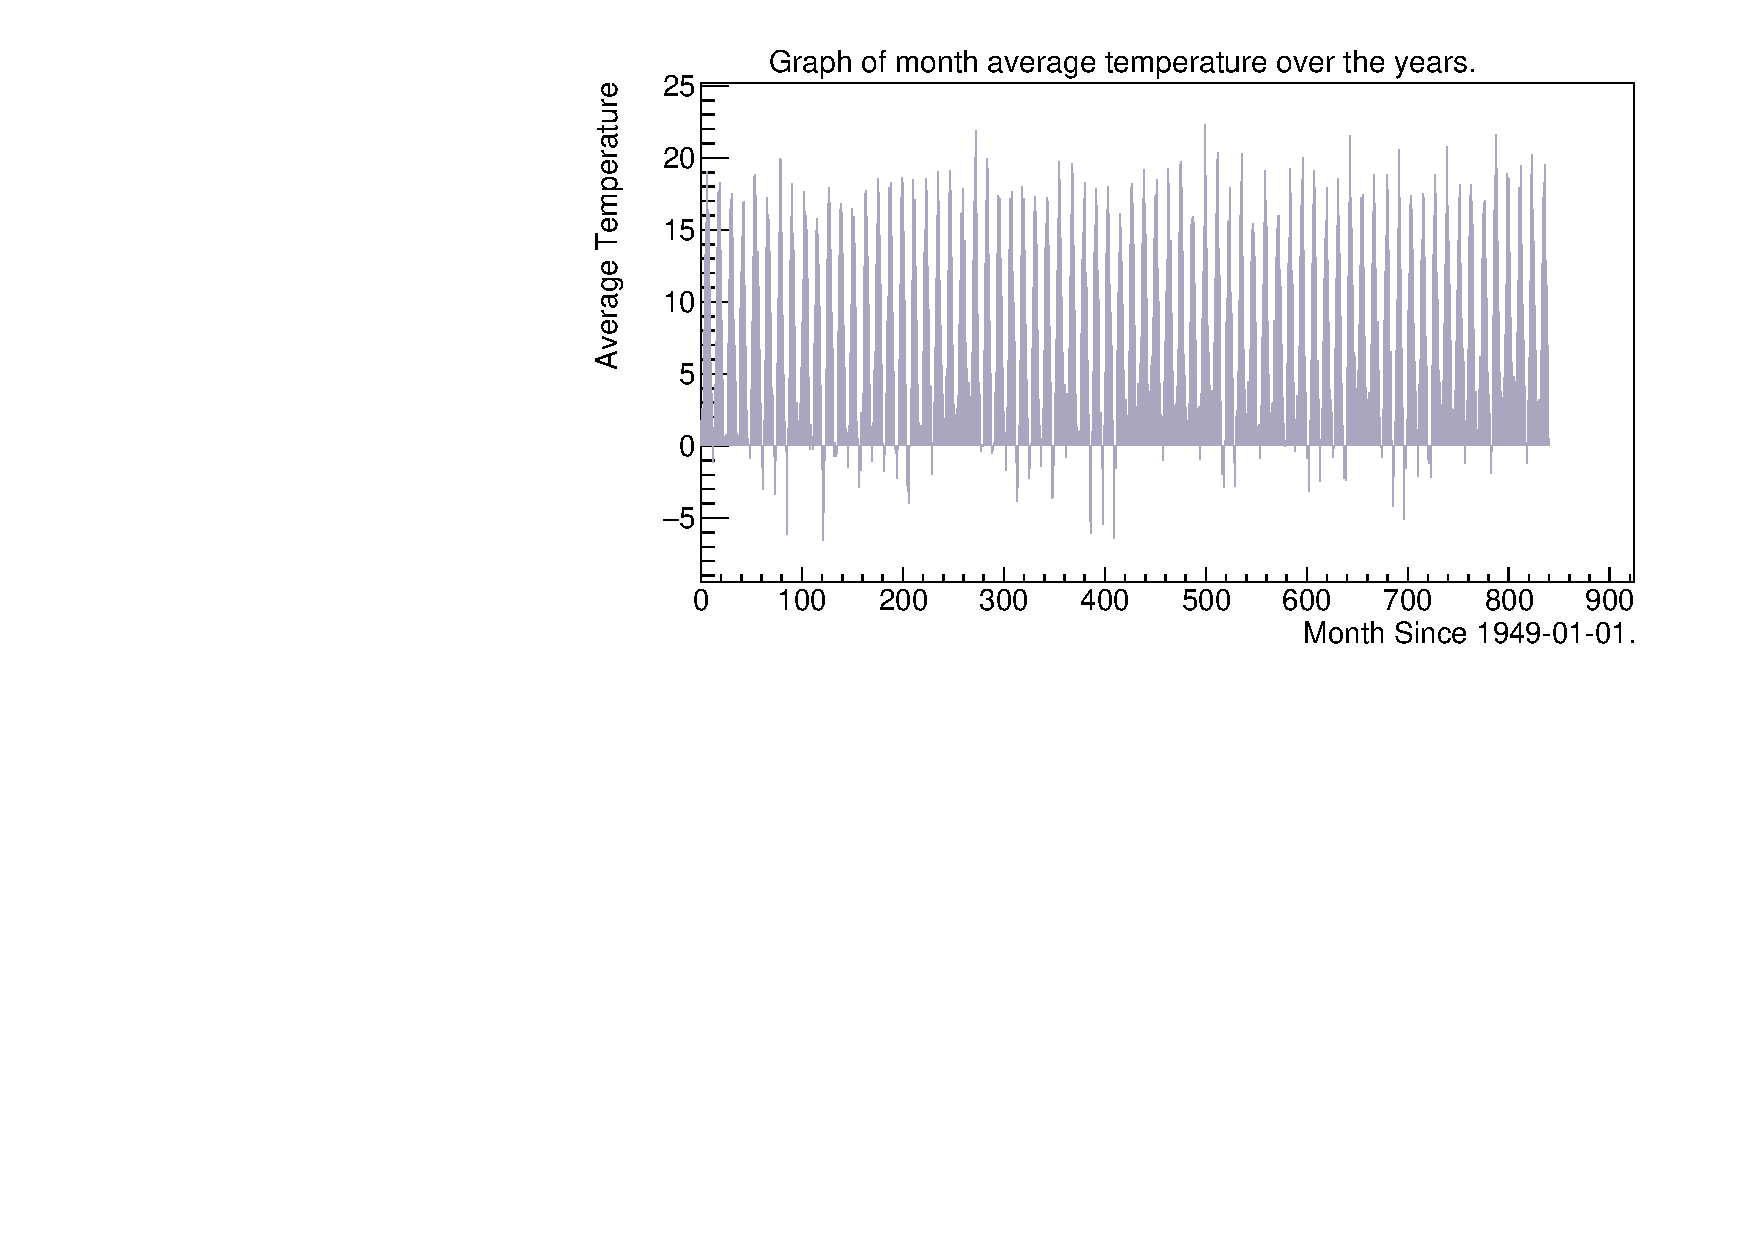
\includegraphics[width=\textwidth]{monthlyAverageTemperatureLund.pdf}
            \caption{Monthly average temperature from 1949-01-01 in Lund.}
            \label{fig:monthlyLund}
    \end{subfigure}
    \hfill
    \begin{subfigure}{0.45\textwidth}
            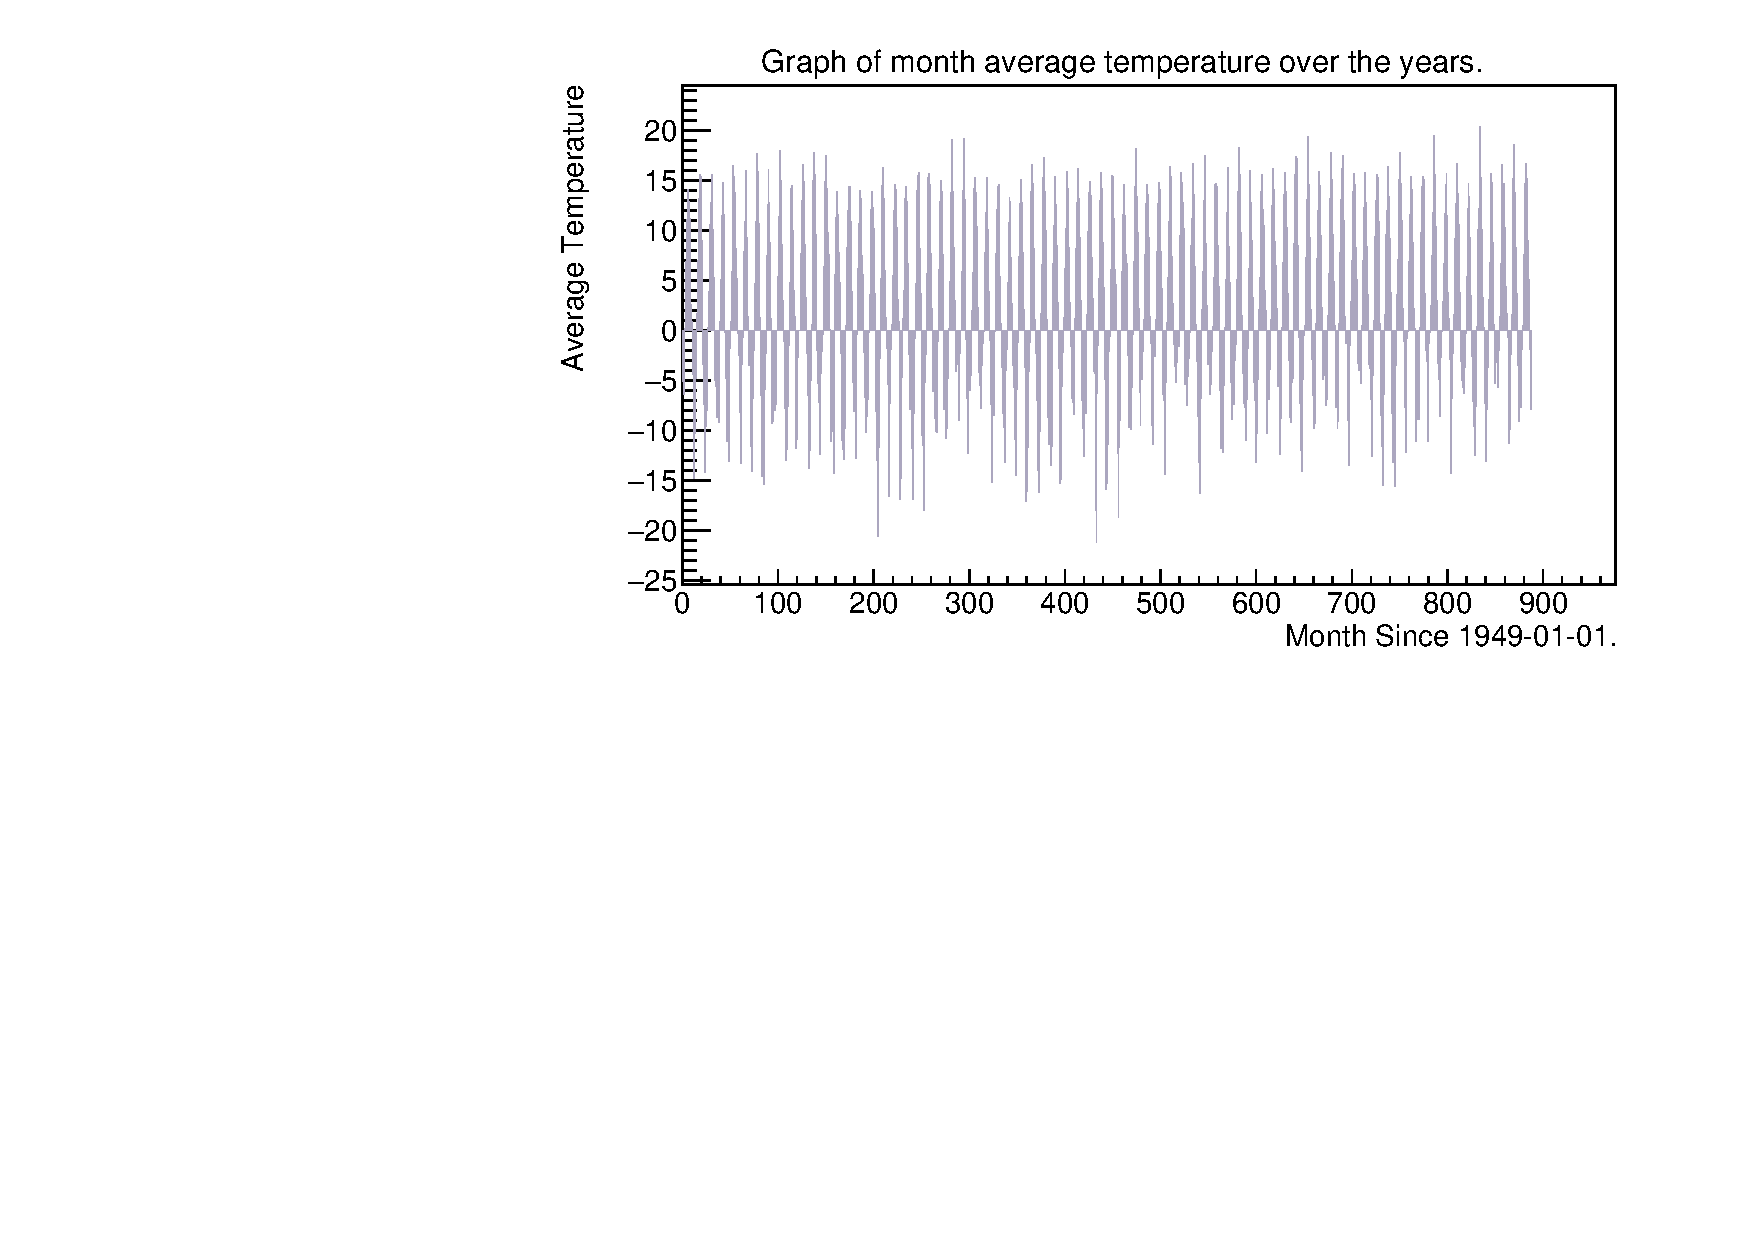
\includegraphics[width=\textwidth]{monthlyAverageTemperatureLulea.pdf}
            \caption{Monthly average temperature from 1949-01-01 in Luleå.}
            \label{fig:monthlyLulea}
    \end{subfigure}
    \caption{Monthly average temperatures in Lund and Luleå.}
    \label{fig:monthlyTemp}
\end{figure}
\vspace{-0.3cm}

The second result was from looking at the temperature difference between the two cities as Lund - Luleå.
\begin{figure}[h!]
    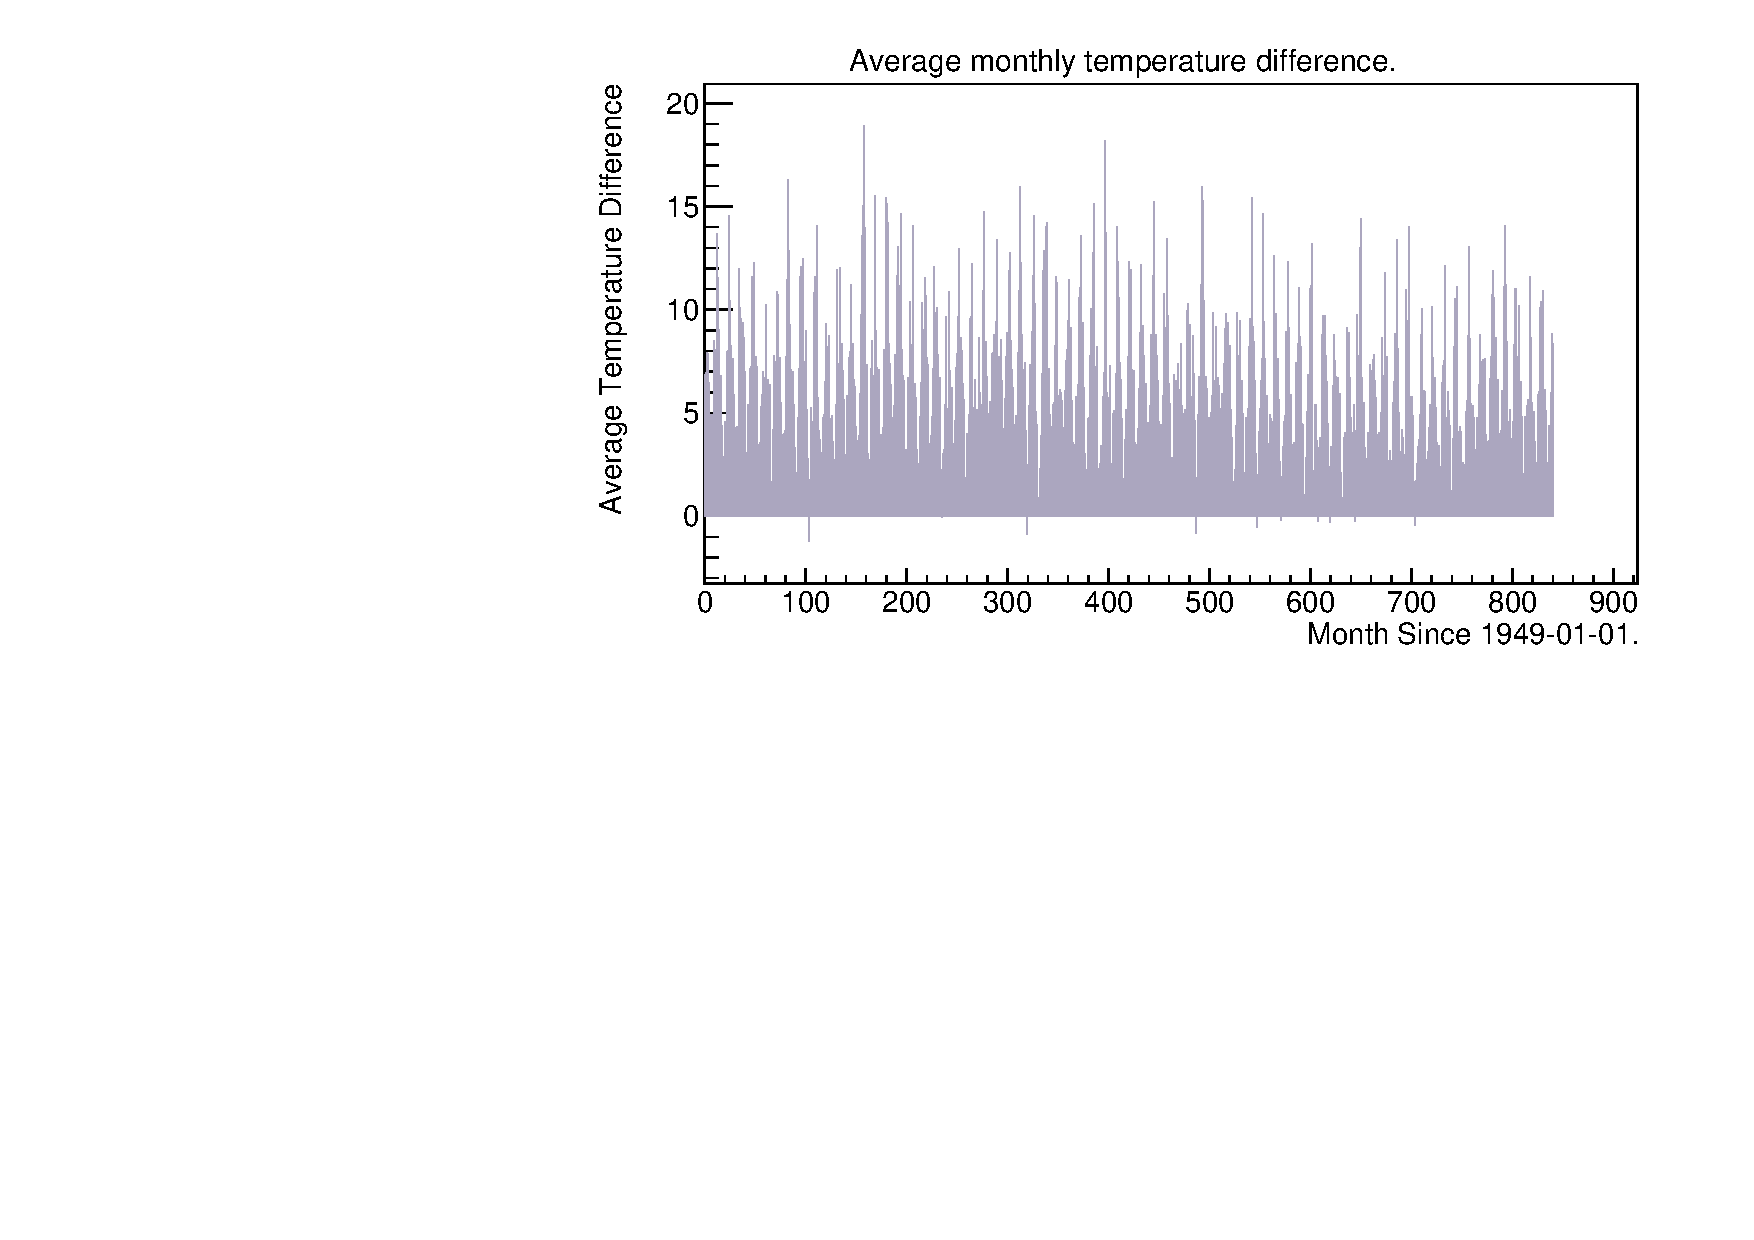
\includegraphics[width=0.45\textwidth]{temperaturedeltaLundLulea.pdf}
    \caption{Temperature delta Lund - Luleå from 1949-01-01.}
    \label{fig:monthlyDelta}
\end{figure}
\vspace{-0.3cm}

The final result of the sub-project is the average temperature delta between the cities for each month. This result shows that the temperature difference is greatest in the cold month and goes to its minimum during July. The reason for this is that as already discussed before the temperature in Lund stays relatively consistently positive throughout the year while Luleå changes drastically during the year meaning that the temperature difference is smallest during the warm month of the year.
\begin{figure}[h!]
    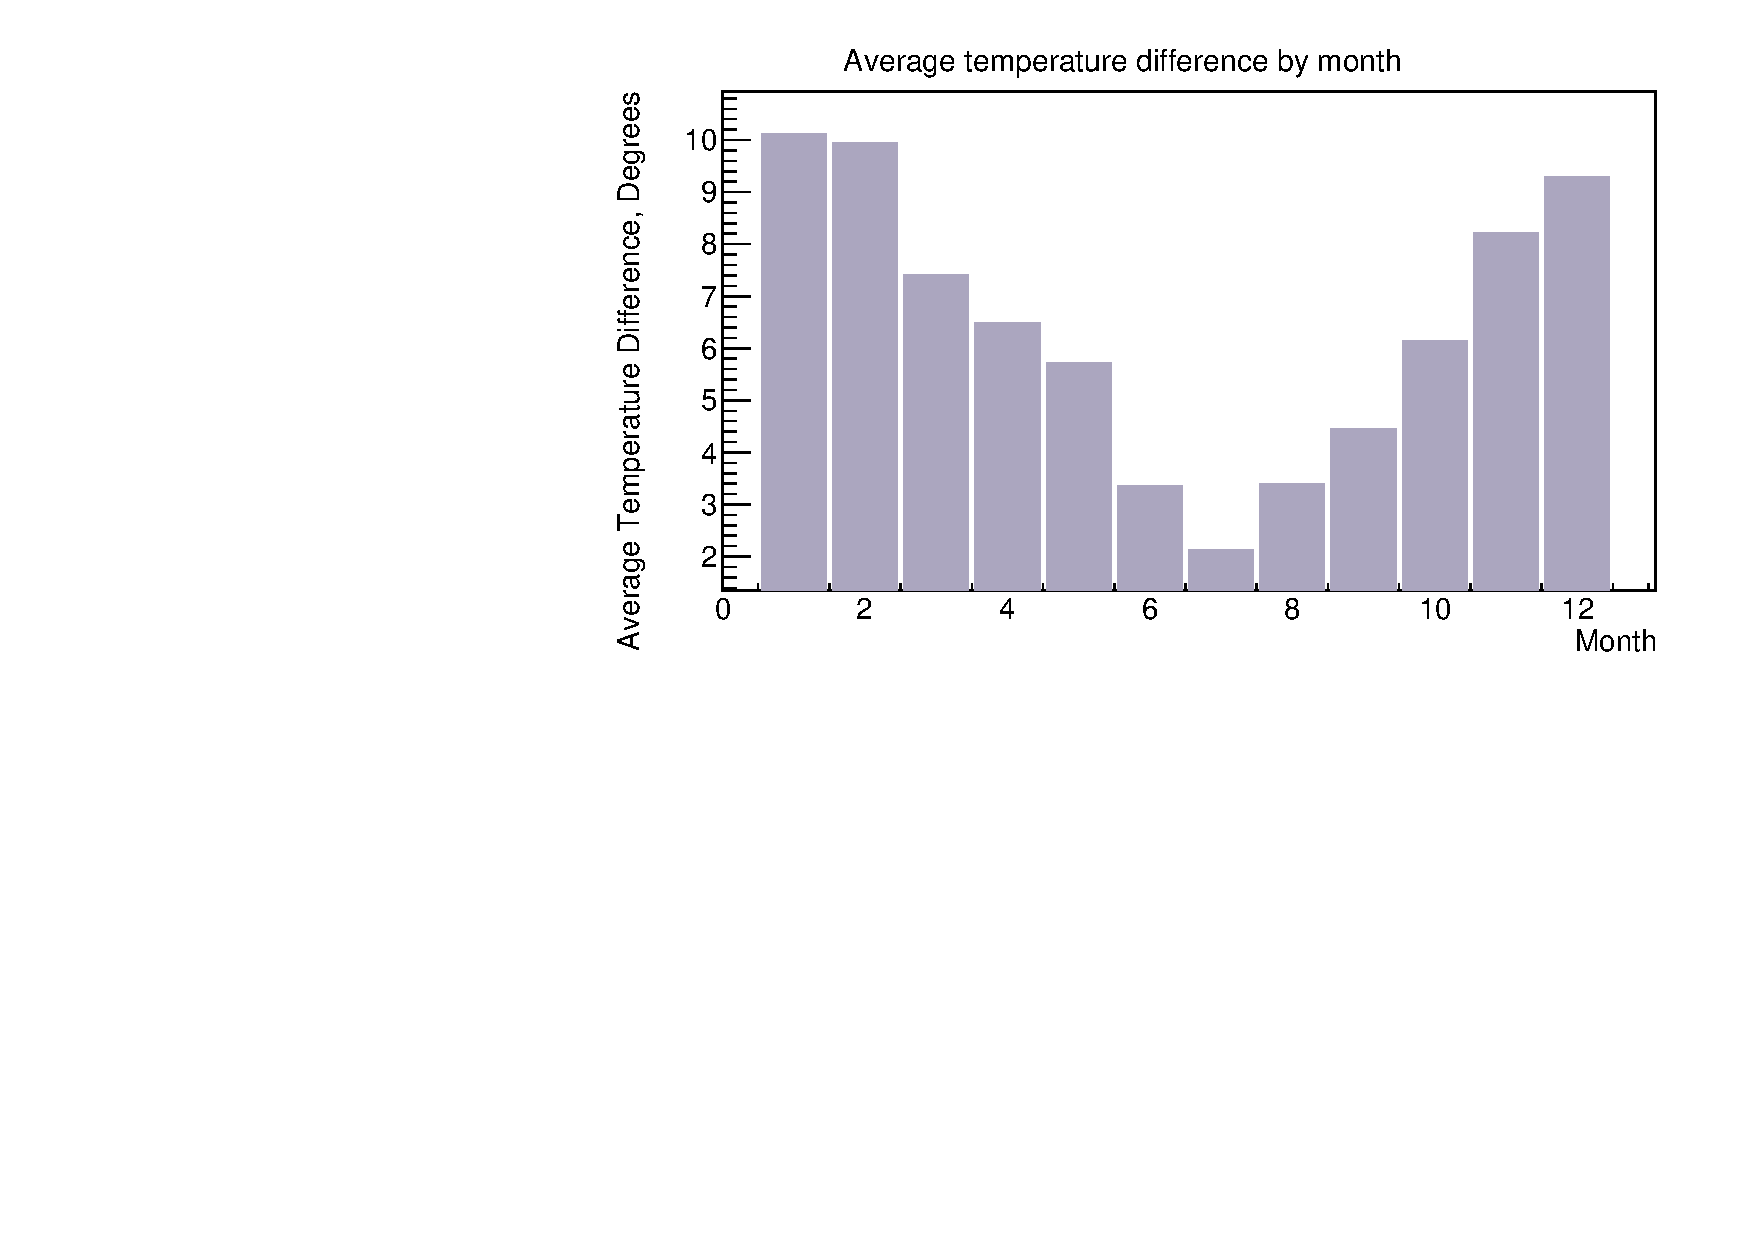
\includegraphics[width=0.45\textwidth]{tempDeltaByMonth.pdf}
    \caption{Monthly Temperature Delta.}
    \label{fig:tempDelta}
\end{figure}
\vspace{-0.8cm}


\section{Hottest and coldest days over the years}

This sub projects goal was to try to find out the day which was likeliest to be the hottest or coldest day by analyzing data provided by SMHI. Specifically the data regarding Lund, Uppsala and Luleå during the time period 1949-2023. The approach to this goal was to take out the days which had the hottest/coldest temperature from the data and then process it so that it could be entered into a plot after which one could analyze the results. The processing was done with both a bash script and  and c++ functions. The plotting was done using the ROOT framwork.
Similar to previous sections there will be three sections, the first one discussing the data preparation, the second one discussing the C++ script and the ROOT plotting and the last one discussing the results.
\vspace{-0.3cm}

\subsection{Data pre processing}
 The data was, after being cleaned using bash script mentioned above, run through another bash script called MaxMinPerYear.sh. This script picks goes through every year after 1949 and picks out the hottest and coldest days from these years. It also removes the year from the data as only the month and day matters for our purpose. Since bash doesn't handle numbers the script picks out temperatures for the relevant year and sorts them which allows us to bypass any need to compare numbers as the bottom and top result is the highest and lowest temperatures.
 \vspace{-0.5cm}

 \subsection{C++ and plotting}
The data processing using C++ is done using the functions MinMax map and MinMax hist fill in
MinMaxTemp. The first function takes a csv file cleaned using aforementioned method as input. The function then converts the dates into one of the numbers between 1-366 corresponding to the date and returns it as an <int int> map. The second function takes the map from the first function and adds the data into a histogram. The plotting is then done by MinMax hist draw and the plot is saved as a pdf called MinMax.pdf. 
\vspace{-0.3cm}
 
 \subsection{Results}
The resulting plots are histograms over the warmest and coldest days over the years since 1949 in Luleå, Uppsala and Lund. Looking at the histograms one can see that for luleå the hottest day is about 27:th of july and the coldest is the 8:th of January. On the histogram for uppsala the hottest day is the 9:th of July and the 1:st of August and the coldest day 29:th of december. For the Lund histogram one can see that the hottest day is first of July and 7:th of August and the coldest day the 28:th and 31:st of December.
\vspace{-0.4cm}

\begin{figure}[h!]
    \begin{subfigure}{0.45\textwidth}
            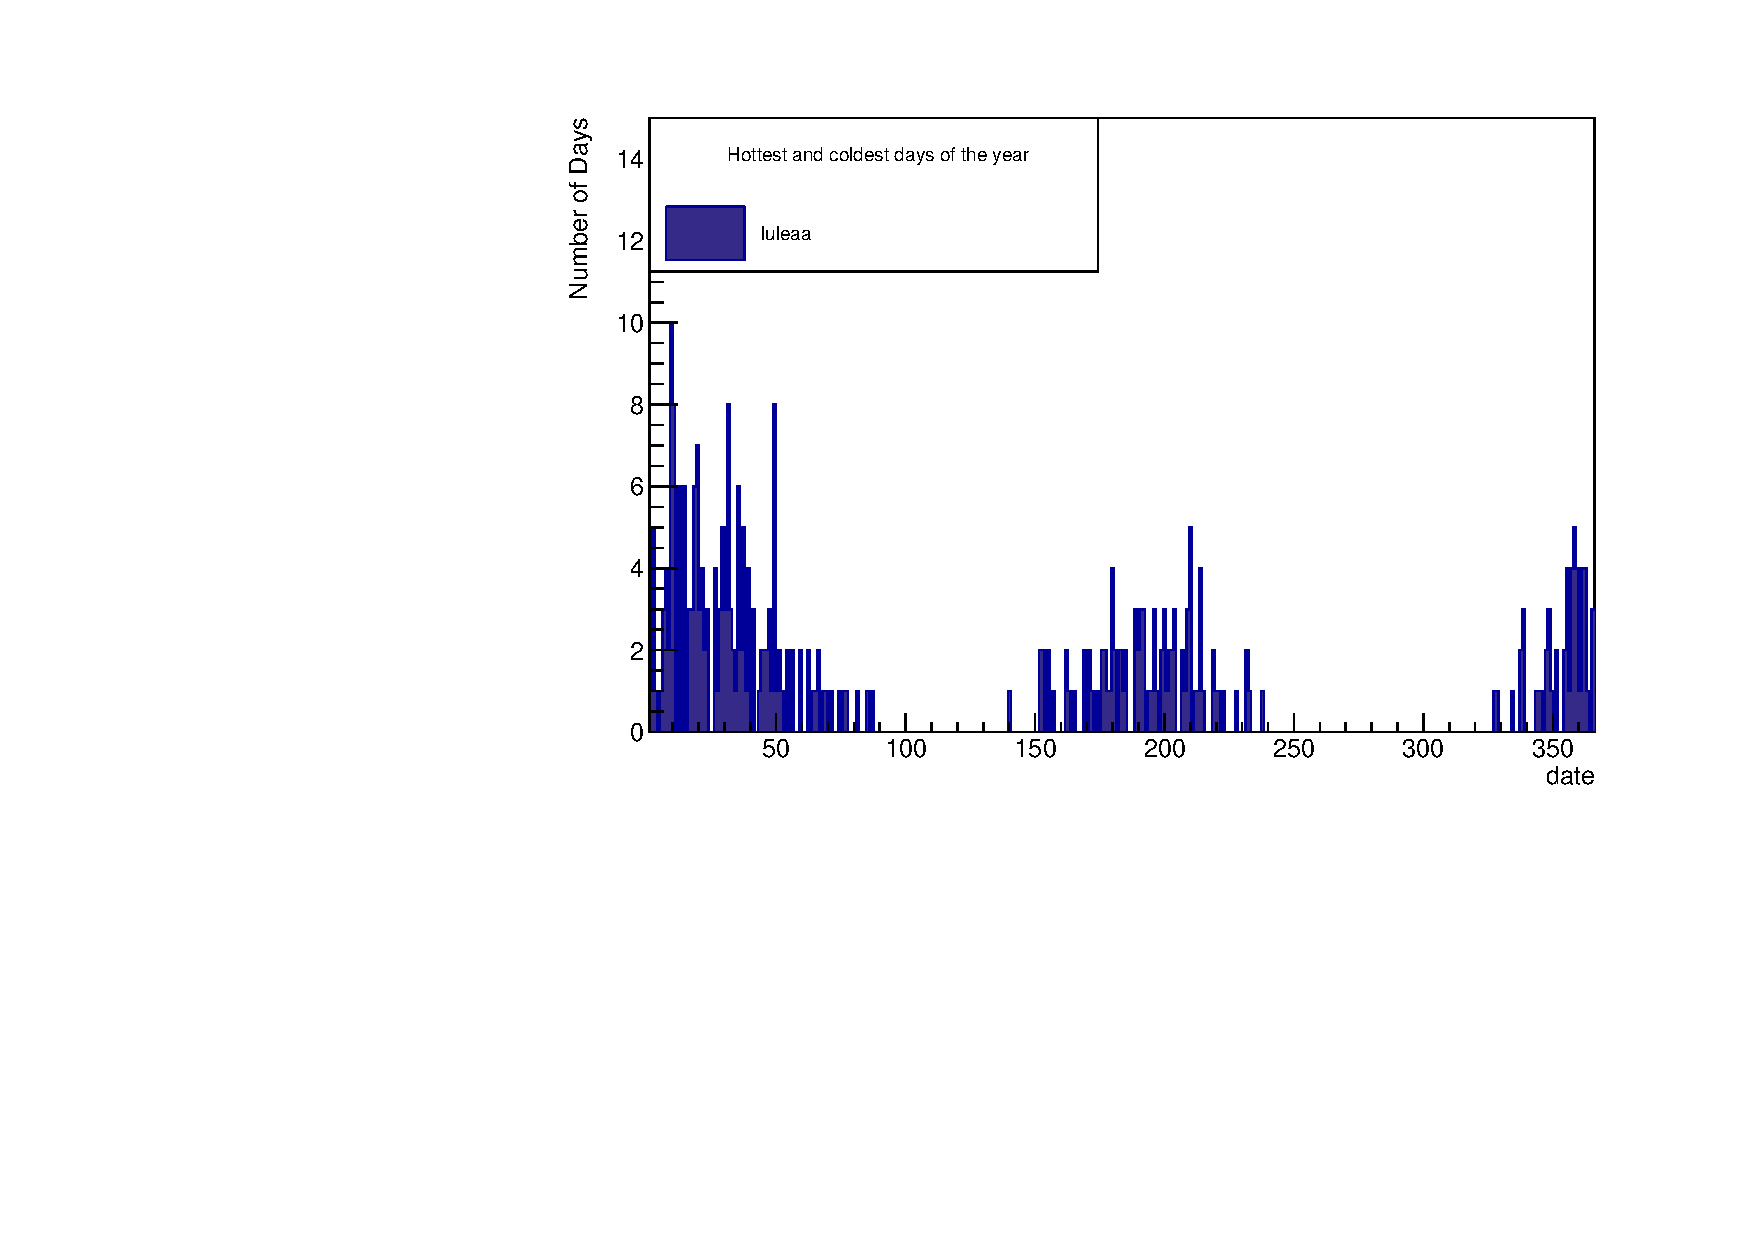
\includegraphics[width=\textwidth,trim= 0 0 0 0.6cm,clip]{MinMaxLuleaa.pdf}
            \vspace{-0.6cm}
            \caption{Maximum and Minimum temperature Luleå}
            \label{fig:MinMaxLuleå}
    \end{subfigure}
    
    \vspace{-0.0cm}
    \begin{subfigure}{0.45\textwidth}
            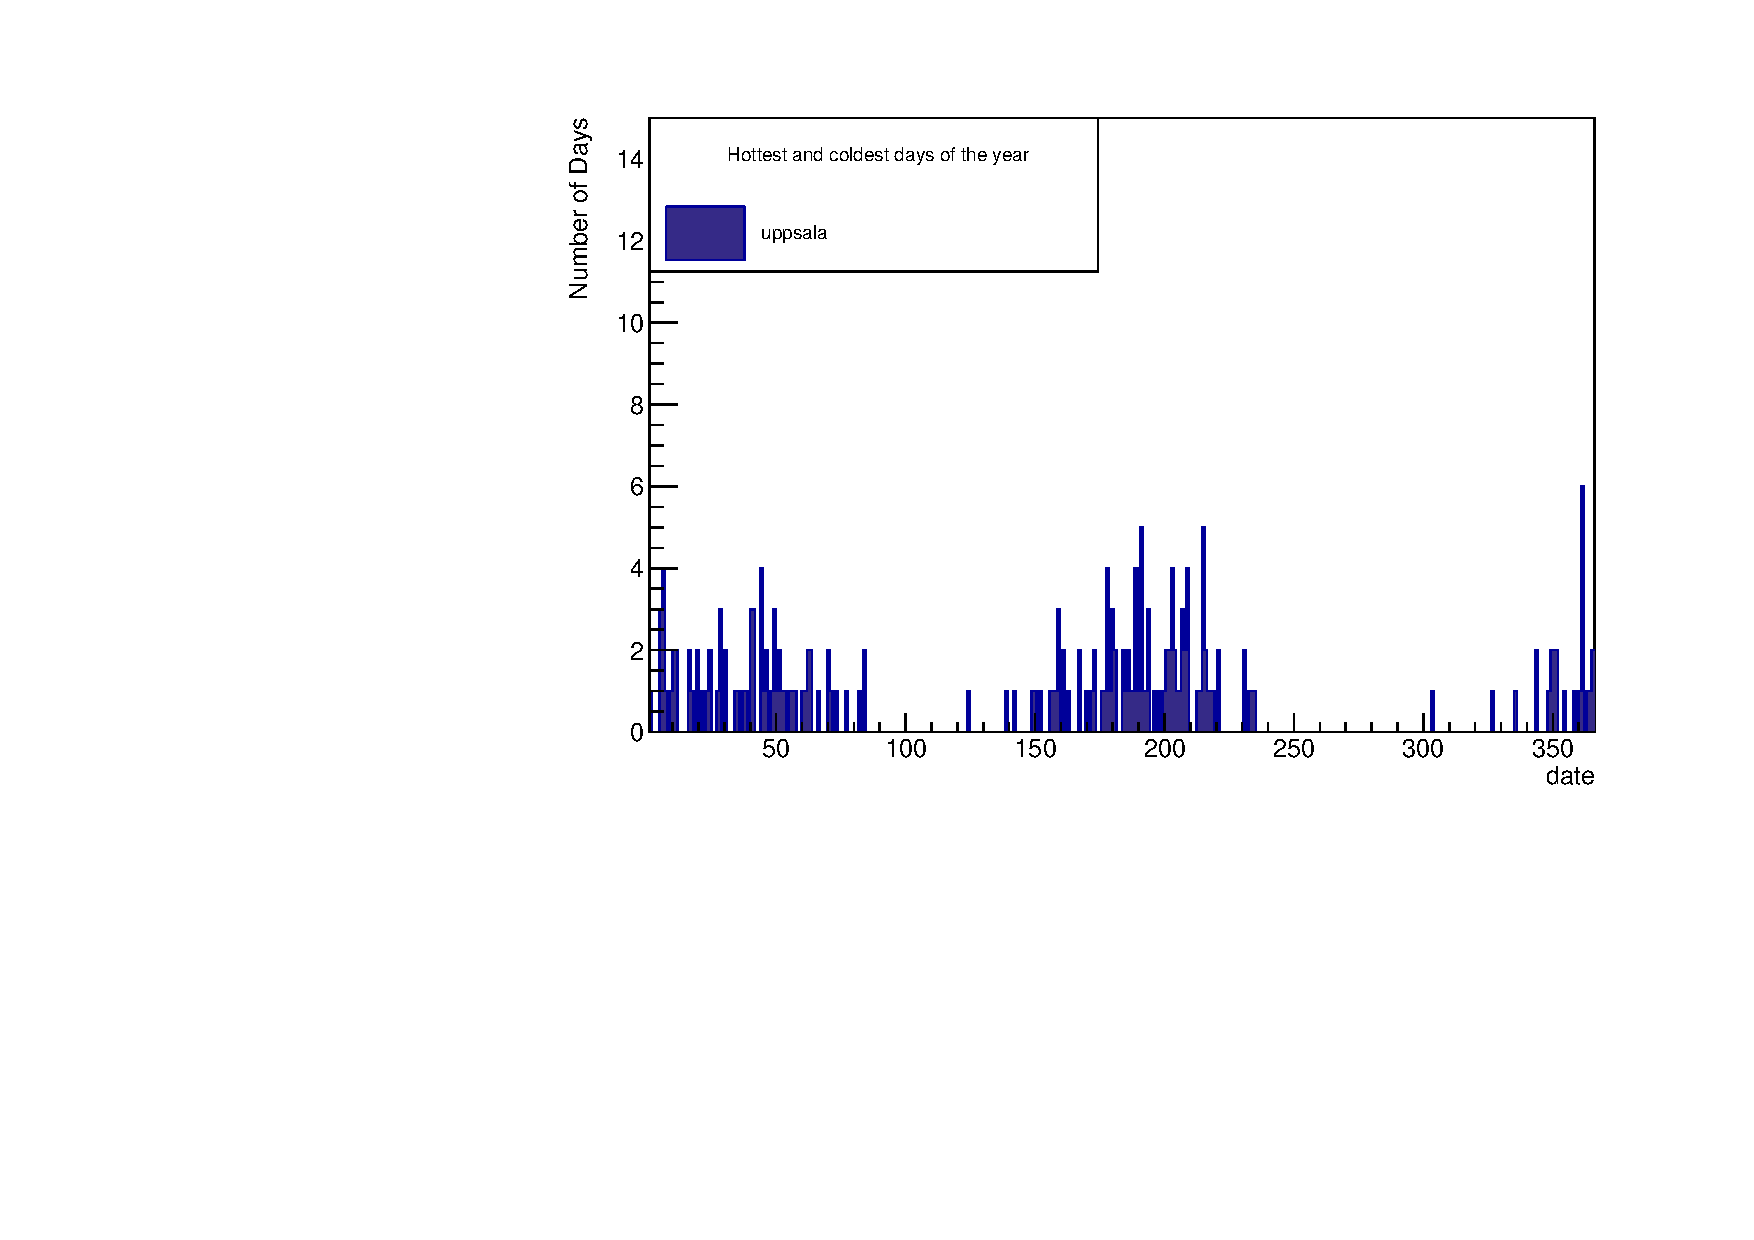
\includegraphics[width=\textwidth,trim= 0 0 0 0.6cm,clip]{MinMaxuppsala.pdf}
            \vspace{-0.6cm}
            \caption{Maximum and Minimum temperature Uppsala}
            \label{fig:MinMaxUppsala}
    \end{subfigure}
    \begin{subfigure}{0.45\textwidth}
            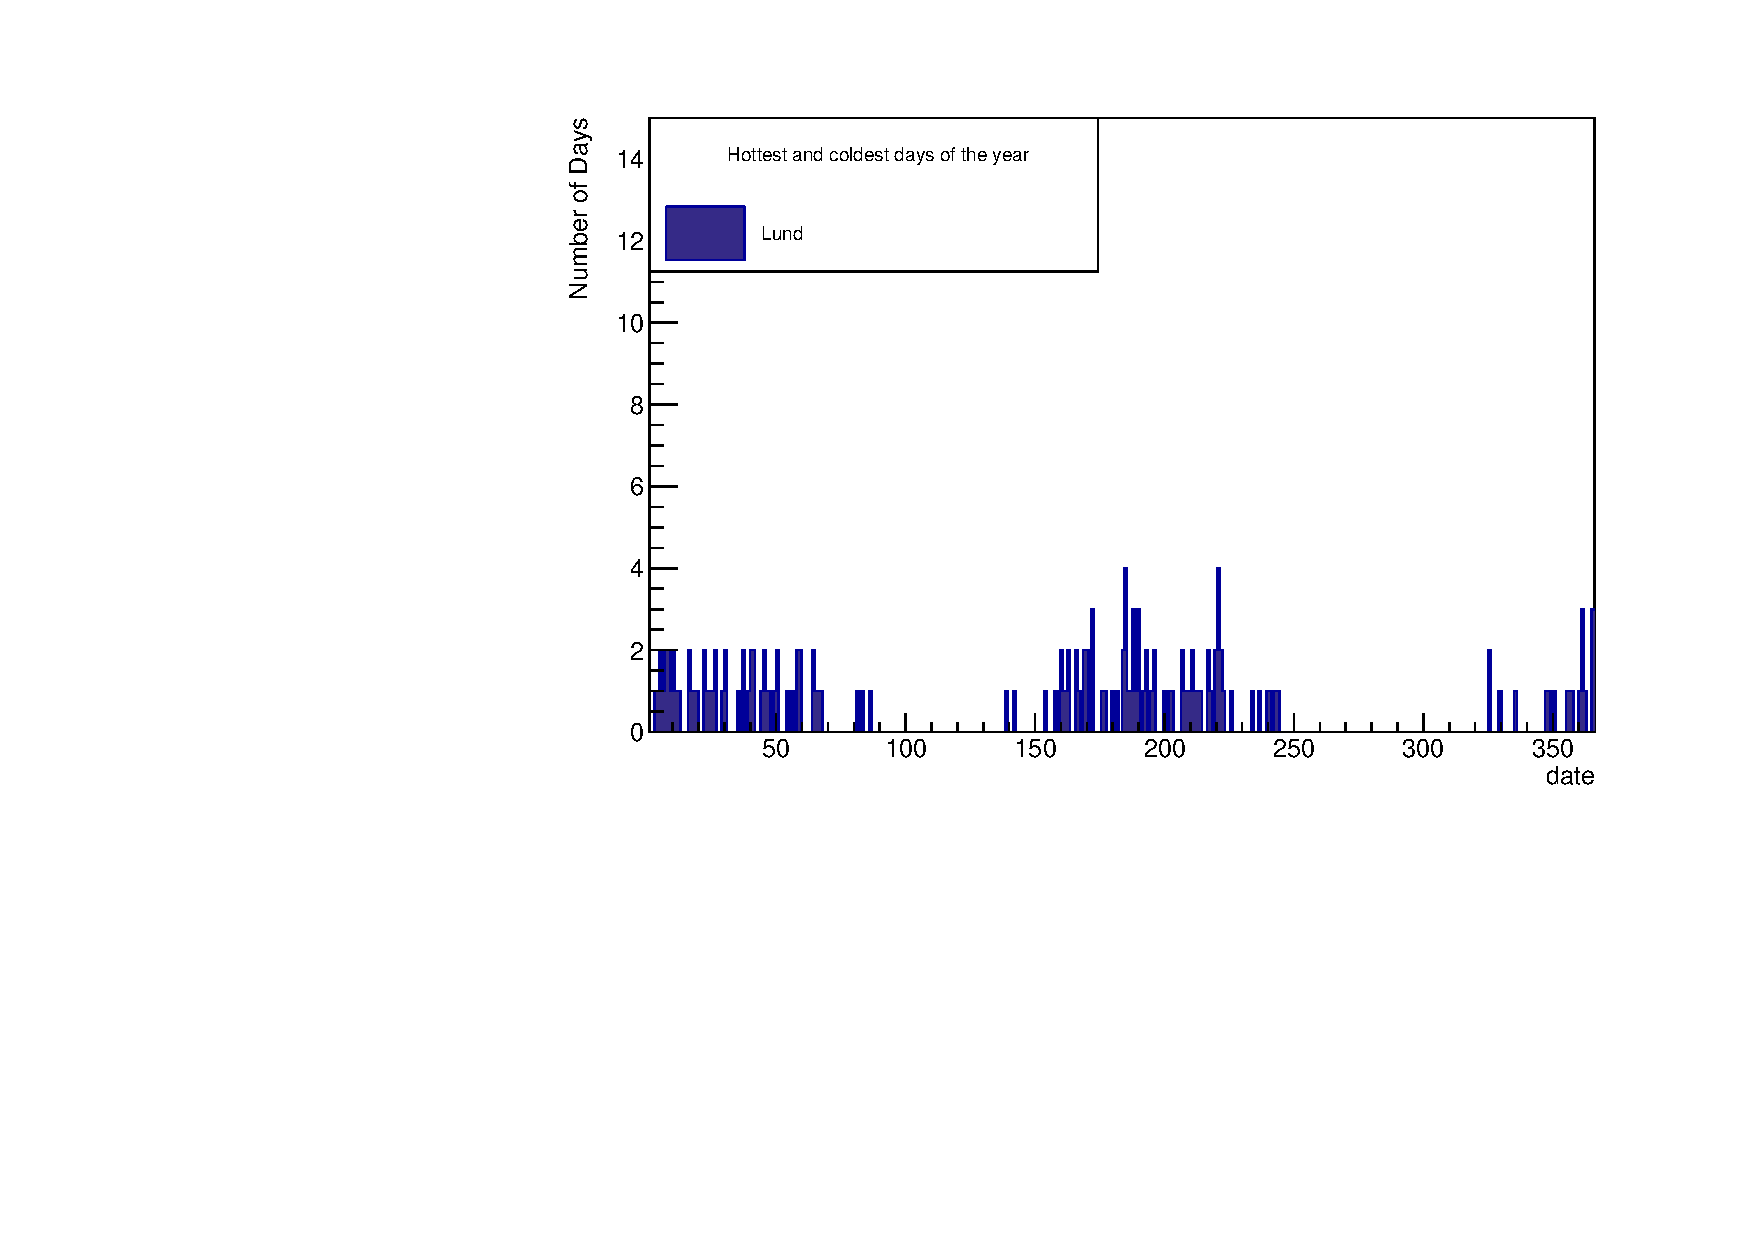
\includegraphics[width=\textwidth,trim= 0 0 0 0.6cm,clip]{MinMaxLund.pdf}
            \vspace{-0.6cm}
            \caption{Maximum and Minimum temperature Lund}
            \label{fig:MinMaxLund}
    \end{subfigure}

\end{figure}
As one can see from the figures the farther south you go the harder it gets to predict the hottest and coldest days which is interesting. The one consistent pattern that can be spotted is that the end of July and beginning of August is the likeliest to contain the days that are the hottest and the whole month of January is the likeliest to contain the coldest day by far.


\section{Conclusions and Outlook}

\subsection{Number of Winter Days}
The key findings for the number of winter days subproject were the decreasing moving averages, which are an indication of global warming. This feature was clear in the Uppsala and Luleå datasets, but much harder to discern in the Lund dataset. Concerning the relative number of winter days, using Luleå as a reference, Lund showed higher variations than Uppsala. 2009 was the year with the highest number of winter days, during the time period 1964-2022, in both the Lund and Uppsala datasets. This year also had the highest relative number of winter days when comparing Lund and Uppsala to Luleå. Possible improvements to the data analysis process include replacing the maps with a new class containing the year and number of winter days as variables. This would make the code far more transparent for any potential readers. Another improvement would be to not have a hard-coded time period, which would make the program far less case specific.

\subsection{Average monthly temperature}
The results for the average monthly temperature part of the project turned out nicely. The main takeaway in terms of the analysis was the fact that the temperature difference between Lund and Luleå is lowest during July, the hottest month of the year and increases during the colder month. The data analysis tooling developed for this part of the experiment can work on any two data sets that were formatted in the same way and have a common time period that could be used for analysis. As a possible improvement for the tooling the performance of the C++ program could likely be improved significantly if, instead of a large amount of functions traversing through the maps and passing them to one another, there would be a single function that does the calculations and averaging straight away.

\subsection{Hottest and coldest days}
While finding a date where the temperature was likely the hottest or the coldest was not successful it was still narrowed down to a small area of dates that were more likely to be the hottest. Some interesting patterns were found though. All of the datasets had a hot peak near late June and early August and the coldest day was more likely to be close to new years eve. Another very interesting pattern is that the further south we go the harder it gets to predict peak and bottom temperature. This could be due to Lund not having as many measurements as the other datasets though.
There are some improvements to be made such as highlighting which part is the hottest and which is the coldest in the histograms. Another improvement could be to add markers to more easily see the peaks on the histogram and also making the date easier to read. It is currently hard to say a date with precision without digging in the data. The code in itself could be improved by changing the if statements to switch cases and removing legacy code which would improve legibility. It might also be interesting to create a function that could create a histogram that collects data from several datasets creating a combined map in order to get a highest and lowest temperature over the entire country.

\begin{thebibliography}{99}

\bibitem{smhi}
Sveriges meteorologiska och hydrologiska institut, \textit{Ladda ner meteorologiska observationer}, SMHIs öppna data, URL: https://www.smhi.se/data/meteorologi/ladda-ner-meteorologiska-observationer/\#param=airtemperature-Instant,stations=core .
\end{thebibliography}

\end{document}
%
% ****** End of file apstemplate.tex ******